\section*{Introduction}

A distributed system is made highly available when individual servers are
allowed to operate independently without failure-prone, high latency
coordination.
The independent nature of the server's behavior means that it can immediately
respond to client requests, but that it does so from a limited, local
perspective which may be inconsistent with another server's response.
If individual servers in a system were allowed to remain wholly independent,
individual requests from clients to different servers would create a lack of
order or predictability, a gradual decline into inconsistency, e.g. the
system would experience \textit{entropy}.
To combat the effect of entropy while still remaining highly available,
servers engage in periodic background \textit{anti-entropy
  sessions}~\cite{terry_session_1994}.

Anti-entropy sessions synchronize the state between servers ensuring that,
at least briefly, the local state is consistent with a portion of the global
state of the system.
If all servers engage in anti-entropy sessions, the system is able to make
some reasonable guarantees about the timeliness of responses; the most famous
of which is that without requests the system will become
consistent, eventually.
More specifically, inconsistencies in the form of stale reads can be bound by
likelihoods that are informed by the latency of anti-entropy sessions and the
size of the system~\cite{bailis_quantifying_2014}.
Said another way, overall consistency is improved in an eventually consistent
system by decreasing the likelihood of a stale read, which is tuned by
improving the \textit{visibility latency} of a write, the speed at which a
write is propagated to a significant portion of servers.
This idea has led many system designers to decide that eventual consistency
is ``consistent enough''~\cite{bermbach_eventual_2011,wada_data_2011},
particularly in a data center context where visibility latency is far below
the rate of client requests, leading to practically strong consistency.

Recently there have been two important changes in considerations for the
design of such systems that have led us to re-evaluate propagation speed:
systems are growing, while simultaneously becoming geographically distributed
outside of the datacenter.
Scaling an eventually consistent system to dozens or even hundreds of nodes
increases the radius of the network, which leads to increased noise during
anti-entropy; e.g. the possibility that an anti-entropy session will be
between two already synchronized nodes.
Geographic distribution and extra-datacenter networks increase the latency of
anti-entropy sessions so that inconsistencies become more apparent to
external observers.
Large, geographically-distributed systems are becoming the norm.
From content delivery systems that span the globe, to mobile applications, to
future systems such as automated vehicular networks, all will require
additional consistency guarantees without sacrificing availability.

We propose a new class of adaptive distributed data systems whose replicas
monitor their environment and modify their behavior to optimize consistency.
Anti-entropy uses gossip and rumor spreading to efficiently propagate updates
deterministically without saturating the
network~\cite{haeupler_simple_2015,karp_randomized_2000,moreno_dynamics_2004}.
These protocols use uniform random selection to choose synchronization peers,
which means that a write occurring at one replica is not efficiently
propagated across the network.
We propose the use of \textit{multi-armed bandit}
algorithms~\cite{langford_epoch-greedy_2008,luo_efficient_2017} to optimize
for fast, successful synchronizations by modifying peer selection
probabilities.
The result is a synchronization topology that emerges according to access
patterns and network latency, often localizing communicating replicas to
produce efficient synchronization, lower visibility latency, and increased
consistency.

\section*{System Description}

Our system implements an eventually consistent, in-memory key-value store
that is totally replicated using anti-entropy~\cite{decandia_dynamo:_2007};
a brief sketch of our implementation follows.

\begin{figure}[h]
    \centering
    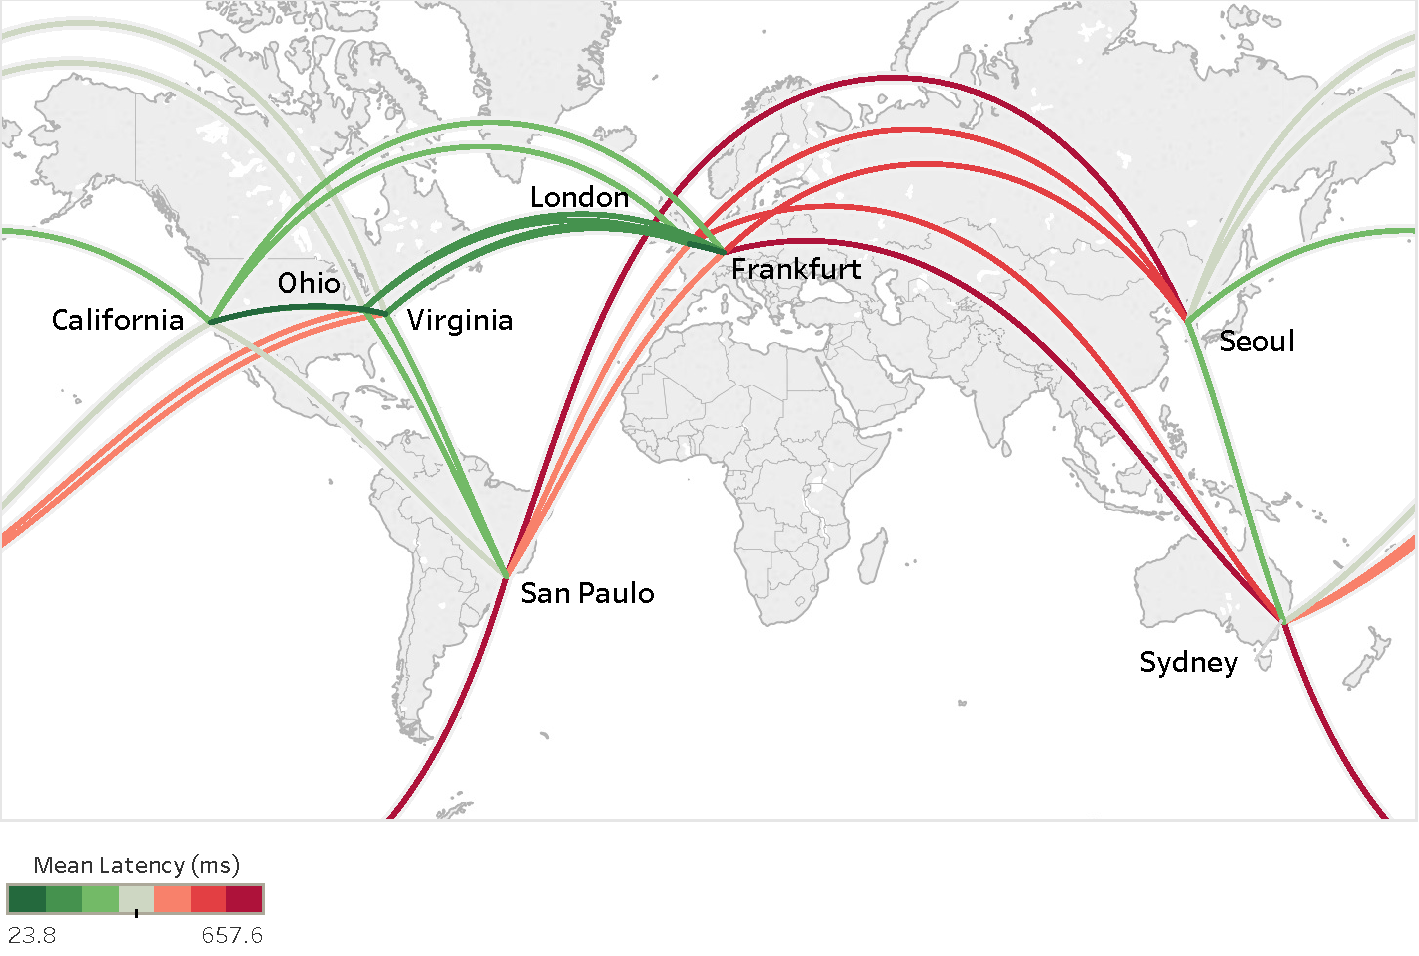
\includegraphics[width=0.5\textwidth]{figures/network}
    \caption{Latencies in a geo-replicated key-value store}
    \label{fig:network}
\end{figure}

\subsection*{Accesses and Consistency}

Clients can \texttt{Put} (write) and \texttt{Get} (read) key-value pairs to
one or more replicas in a single operation.
The set of replicas that responds to a client creates a quorum that must
agree on the state of the operation at its conclusion.
Clients can vary read and write quorum sizes to improve consistency or
availability -- larger quorums reduce the likelihood of stale reads but
smaller quorums respond much more quickly.
In large, geo-replicated systems we assume that clients will prefer to choose
fewer, local replicas to connect with, optimistic that collisions across the
wide-area are rare, e.g. that writes are localized but reads are global.

On \texttt{Put}, the instance of the key-value pair is assigned a
monotonically increasing, conflict-free \textit{version
number}~\cite{almeida_version_2002}.
For simplicity, we assume a fixed number of replicas, therefore each version
is made up of two components: the \textit{update} and \textit{precedence ids}.
Precedence ids are assigned to replicas during configuration, and update ids
are incremented to the largest observed value during synchronization.
As a result, any two versions generated on \texttt{Put} are comparable such
that the \textit{latest} version of the key-value pair is the version with the
largest update id, and in the case of ties, the largest precedence id.

Additional version metadata, including the write's parent version, implements
a virtual object history that allows us to reason about consistency.
Keys can be managed independently, e.g. each key has its own update id
sequence, or all objects can be managed together with a single sequence; in
the latter case, one can construct an ordering history of operations to all
objects.

There are two primary inconsistencies that can occur in this system:
\textit{stale reads} and \textit{forked writes}.
A stale read means that the \texttt{Get} operation has not returned
the globally most recent version of the object.
A forked write, on the other hand, means that there are two branches of the
object history, created by concurrent writes to the same object.
As we will see in the next section, one of these writes will be
\textit{stomped} before it can become fully replicated.
The ideal consistency for a system is represented by a linear object history
without forks.

\subsection*{Anti-Entropy}

Anti-entropy sessions are conducted in a pairwise fashion at a routine
interval to ensure that the network is not saturated with synchronization
requests.
There are two basic forms of synchronization: \textit{push} synchronization
is a fire-and-forget form of synchronization where the remote is sent the
latest version of all objects, whereas \textit{pull} synchronization requests
the latest version of objects and minimizes the size of data transfer.
We have implemented \textit{bilateral} synchronization which combines push
and pull in a two-phase exchange.

Bilateral anti-entropy starts with the initiating replica sending a vector of
the latest local versions of all keys currently stored (this can be optimized
with Merkel trees to make comparisons faster).
The remote replica compares the versions sent by the initiating replica with
its current state and responds with any objects whose version is
\textit{later} than the initiating replica's as well as another version
vector of requested objects that are earlier on the remote.
The initiating remote then replies with the requested objects, completing the
synchronization.
We refer to the first stage of requesting later objects from the remote as
the pull phase, and the second stage of responding to the remote the push
phase.

There are two important things to note about this form of anti-entropy
exchange.
First, this type of synchronization implements a \textit{latest writer wins}
policy.
This means that not all versions are guaranteed to become fully replicated
-- if a later version is written during propagation of an earlier version,
then the earlier version gets stomped by the later version.
If there are two concurrent writes, only one write will become fully
replicated.
Second, the visibility latency is maximized when all replicas choose a remote
synchronization partner that does not yet have the update.
This means that maximal visibility latency is equal to $t\log_3n$, where
$t$ is the anti-entropy interval and $n$ is the number of replicas in the
network.
However, because of stomps and noise created by uniform random selection of
synchronization partners, this latency is never practically achieved.

\section*{Bandit Approaches}

Often used in active and reinforcement machine learning, multi-armed bandits
refer to a statistical optimization procedure that is
designed to find the optimal payout of several choices that each have
different probabilities of reward.
A bandit problem is designed by identifying several ``arms'', so called
because multi-armed bandit refers to pulling slot machine arms, as well as a
reward function that determines how successful the selection of an arm is.
During operation, the bandit uses a \textit{strategy} to select an arm -- the
most common of which is epsilon greedy -- then updates the rewards of the
selected arm, normalized by the number of selections.
The arm with the highest reward value is considered the optimal arm.

Bandits must balance exploration of new arms with possibly better reward
values and exploitation of an arm that has higher rewards than the other.
In the epsilon greedy strategy, the bandit will select the arm with the best
reward with some probability $1-\epsilon$, otherwise it will select any of the
arms with uniform probability.
The smaller $\epsilon$ is, the more the bandit favors exploitation of known
good arms, the larger $\epsilon$ is, the more it favors exploration.
If $\epsilon=1$ then the algorithm is just uniform random selection.
A simple extension of this is annealing epsilon greedy, which starts with a large $\epsilon$, then as the number of trials increases, steadily decreases
$\epsilon$ on a logarithmic scale.

\begin{table}[]
\centering
\begin{tabular}{@{}l c c c @{}}
\toprule
& \textbf{Pull} & \textbf{Push} & \textbf{Total} \\
\midrule
Synchronize at least 1 object & 0.25 & 0.25 & 0.50 \\
Synchronize multiple objects  & 0.05 & 0.05 & 0.10 \\
Latency <= 5ms (local)        & 0.10 & 0.10 & 0.20 \\
Latency <= 100ms (regional)   & 0.10 & 0.10 & 0.20 \\
\midrule
\textit{Total} & \textit{0.50} & \textit{0.50} & \textit{1.00} \\
\bottomrule
\end{tabular}
\caption{Reward Function}
\label{tab:rewards}
\end{table}

Peer selection for anti-entropy is usually conducted with uniform random
selection.
To extend anti-entropy with bandits, we design a selection method whose arms
are remote peers and whose rewards are determined by the success of
synchronization.
The goal of adding bandits to anti-entropy is to optimize selection of peers
such that the visibility latency becomes closer to the optimal propagation
time as a synchronization topology emerges from the bandits.
A secondary goal is to minimize anti-entropy latency by preferring local (in
the same data center) and regional (e.g. on the same continent) connections.

Our reward function favors synchronizations to replicas where the most writes
are occurring by giving higher rewards to anti-entropy sessions that exchange
later versions in either a push or a pull as well as additional rewards if
more than one object is exchanged.
Additionally, the latency of the synchronization RPCs is computed to reward
replicas that are near each other.
The complete reward function is given in Table~\ref{tab:rewards}: for each
phase of synchronization (push and pull), compute the reward as the sum of the
propositions given.
For example if a synchronization results in 3 objects being pulled in 250ms,
and 1 object being pushed in 250ms, the reward is 0.75.

\section*{Experiments}

We conducted experiments using a distributed key-value store totally
replicated across 24 replicas in 8 geographic regions on 5 continents
around the world as shown in Figure~\ref{fig:network}.
Replicas were hosted using AWS EC2 t2.micro instances and were connected to
each other via internal VPCs when in the same region, using external
connections between regions.
The store, called Honu, is implemented in Go 1.9 using gRPC and protocol
buffers for RPC requests; all code is open source and available on GitHub.

The workload on the system was generated by 8 clients, one in each region and
colocated with one of the replicas.
Clients continuously created Put requests for random keys with a unique
prefix per-region (consistency conflicts only occur within a region).
The average throughput generated per-client was 5620.4 puts/second.
Because the mean round trip latency between each region ranged from 23ms to
600ms and synchronization requires at least two round trips, the
anti-entropy delay for these experiments was set to 1 second.
To account for lag between commands sent to replicas in different regions,
the experiment was run for 10 minutes, the workload running for 8 minutes,
offset by one minute from the start.

\begin{figure}[t]
    \centering
    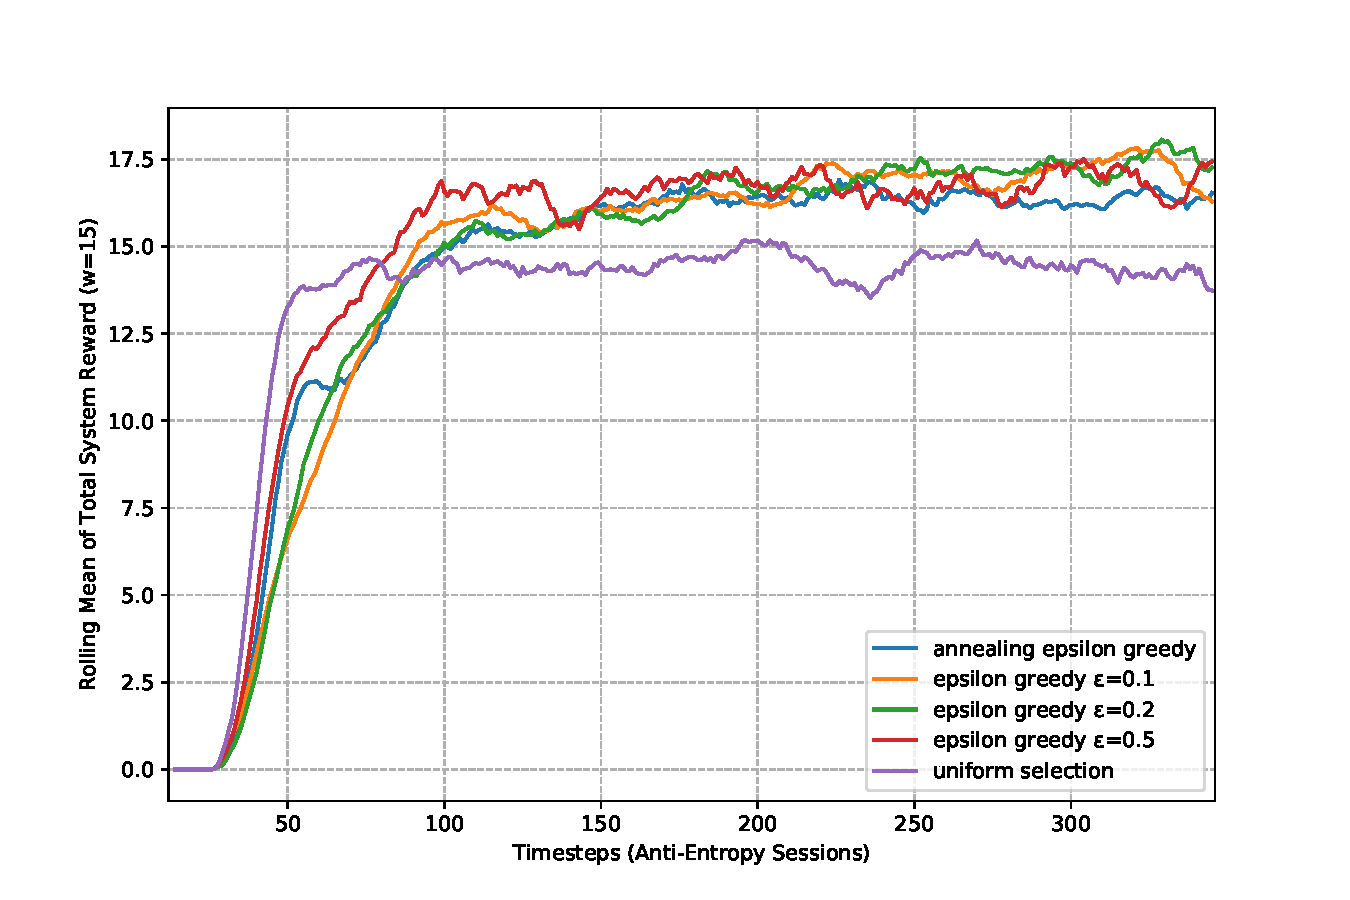
\includegraphics[width=0.5\textwidth]{figures/rewards}
    \caption{Total system rewards over time}
    \label{fig:system_rewards}
\end{figure}

Our first experiments compared uniform random peer selection with epsilon
greedy bandits using $\epsilon \in \{0.1, 0.2, 0.5\}$ as well as an annealing
epsilon greedy bandit.
The total system rewards as a rolling mean over a time window of 15
synchronizations are shown in Figure~\ref{fig:system_rewards}.
The rewards ramp up from zero as the clients come online and start
creating work to be synchronized.
All of the bandit algorithms improve over the baseline of uniform selection,
not only generating more total reward across the system, but also introducing
less variability with lower $\epsilon$ values.
None of the bandit curves immediately produces high rewards as they explore
the reward space; lower $\epsilon$ values may cause exploitation of incorrect
arms, while higher $\epsilon$ values take longer to find optimal topologies.

\begin{figure*}[t]
    \centering
    \minipage{0.5\textwidth}
      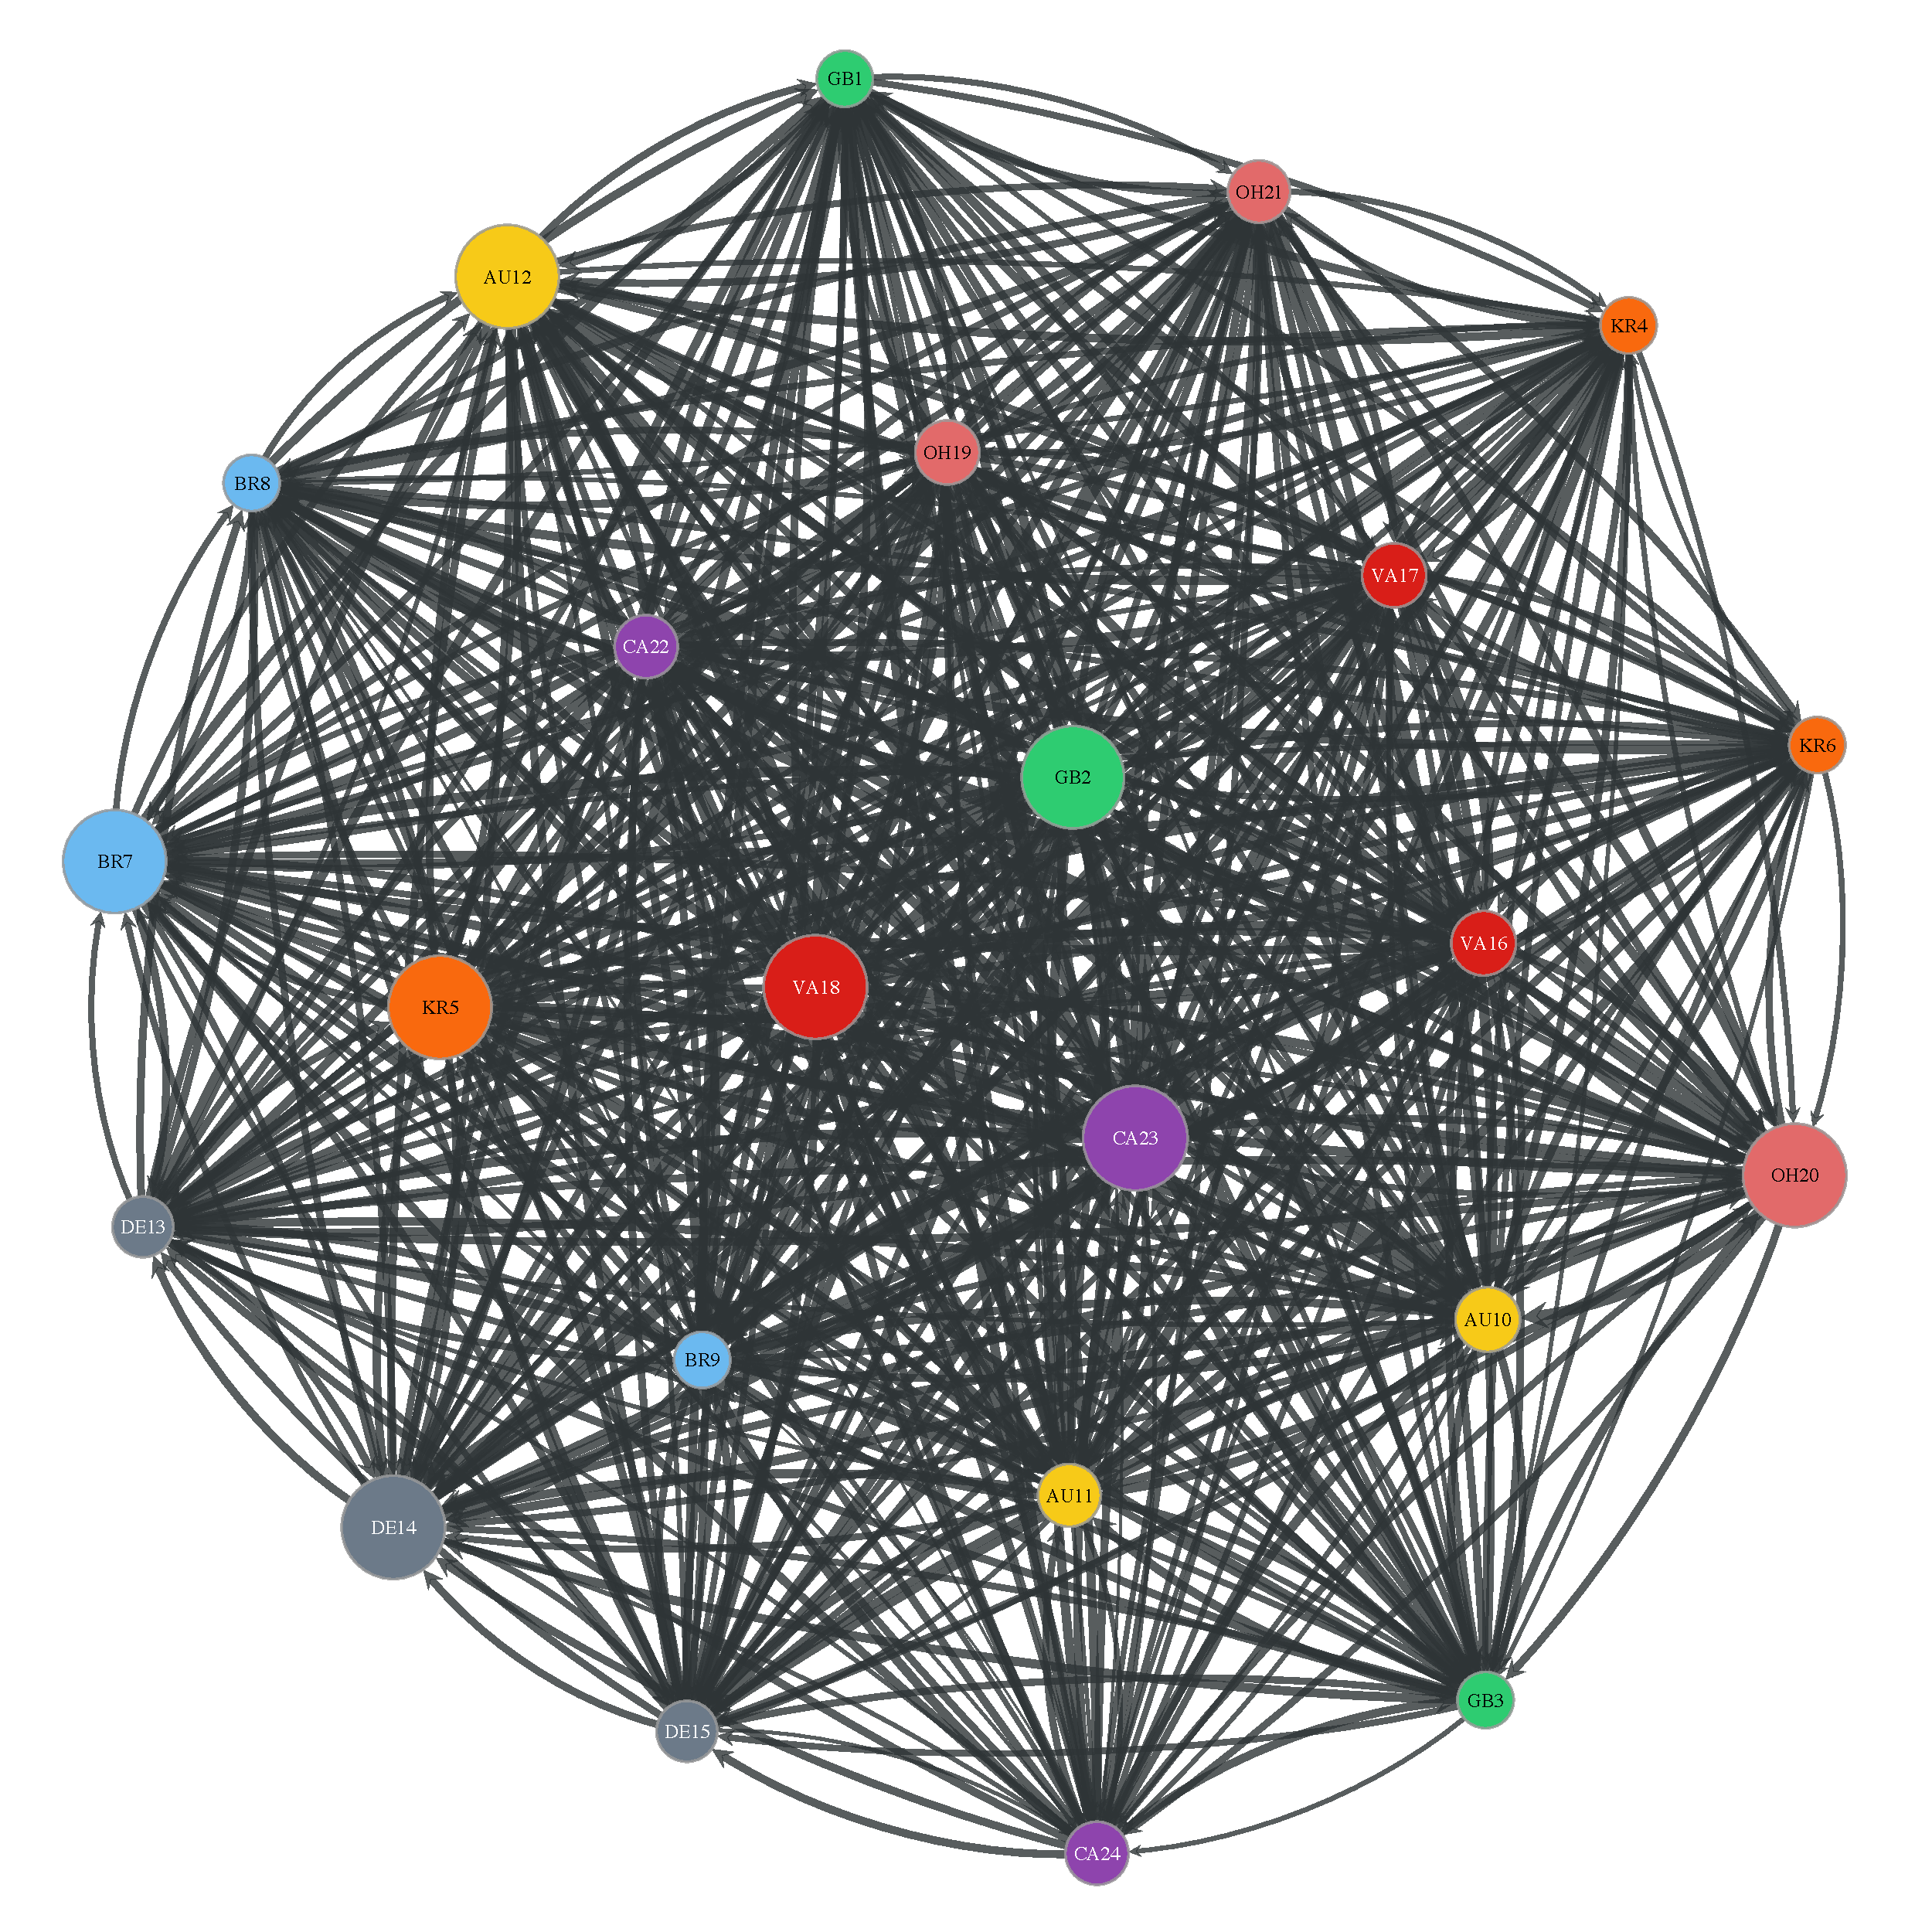
\includegraphics[width=\linewidth]{figures/b-uniform-selection-e1}
      \caption{Uniform Selection}\label{fig:uniform_selection}
    \endminipage\hfill
    \minipage{0.5\textwidth}%
      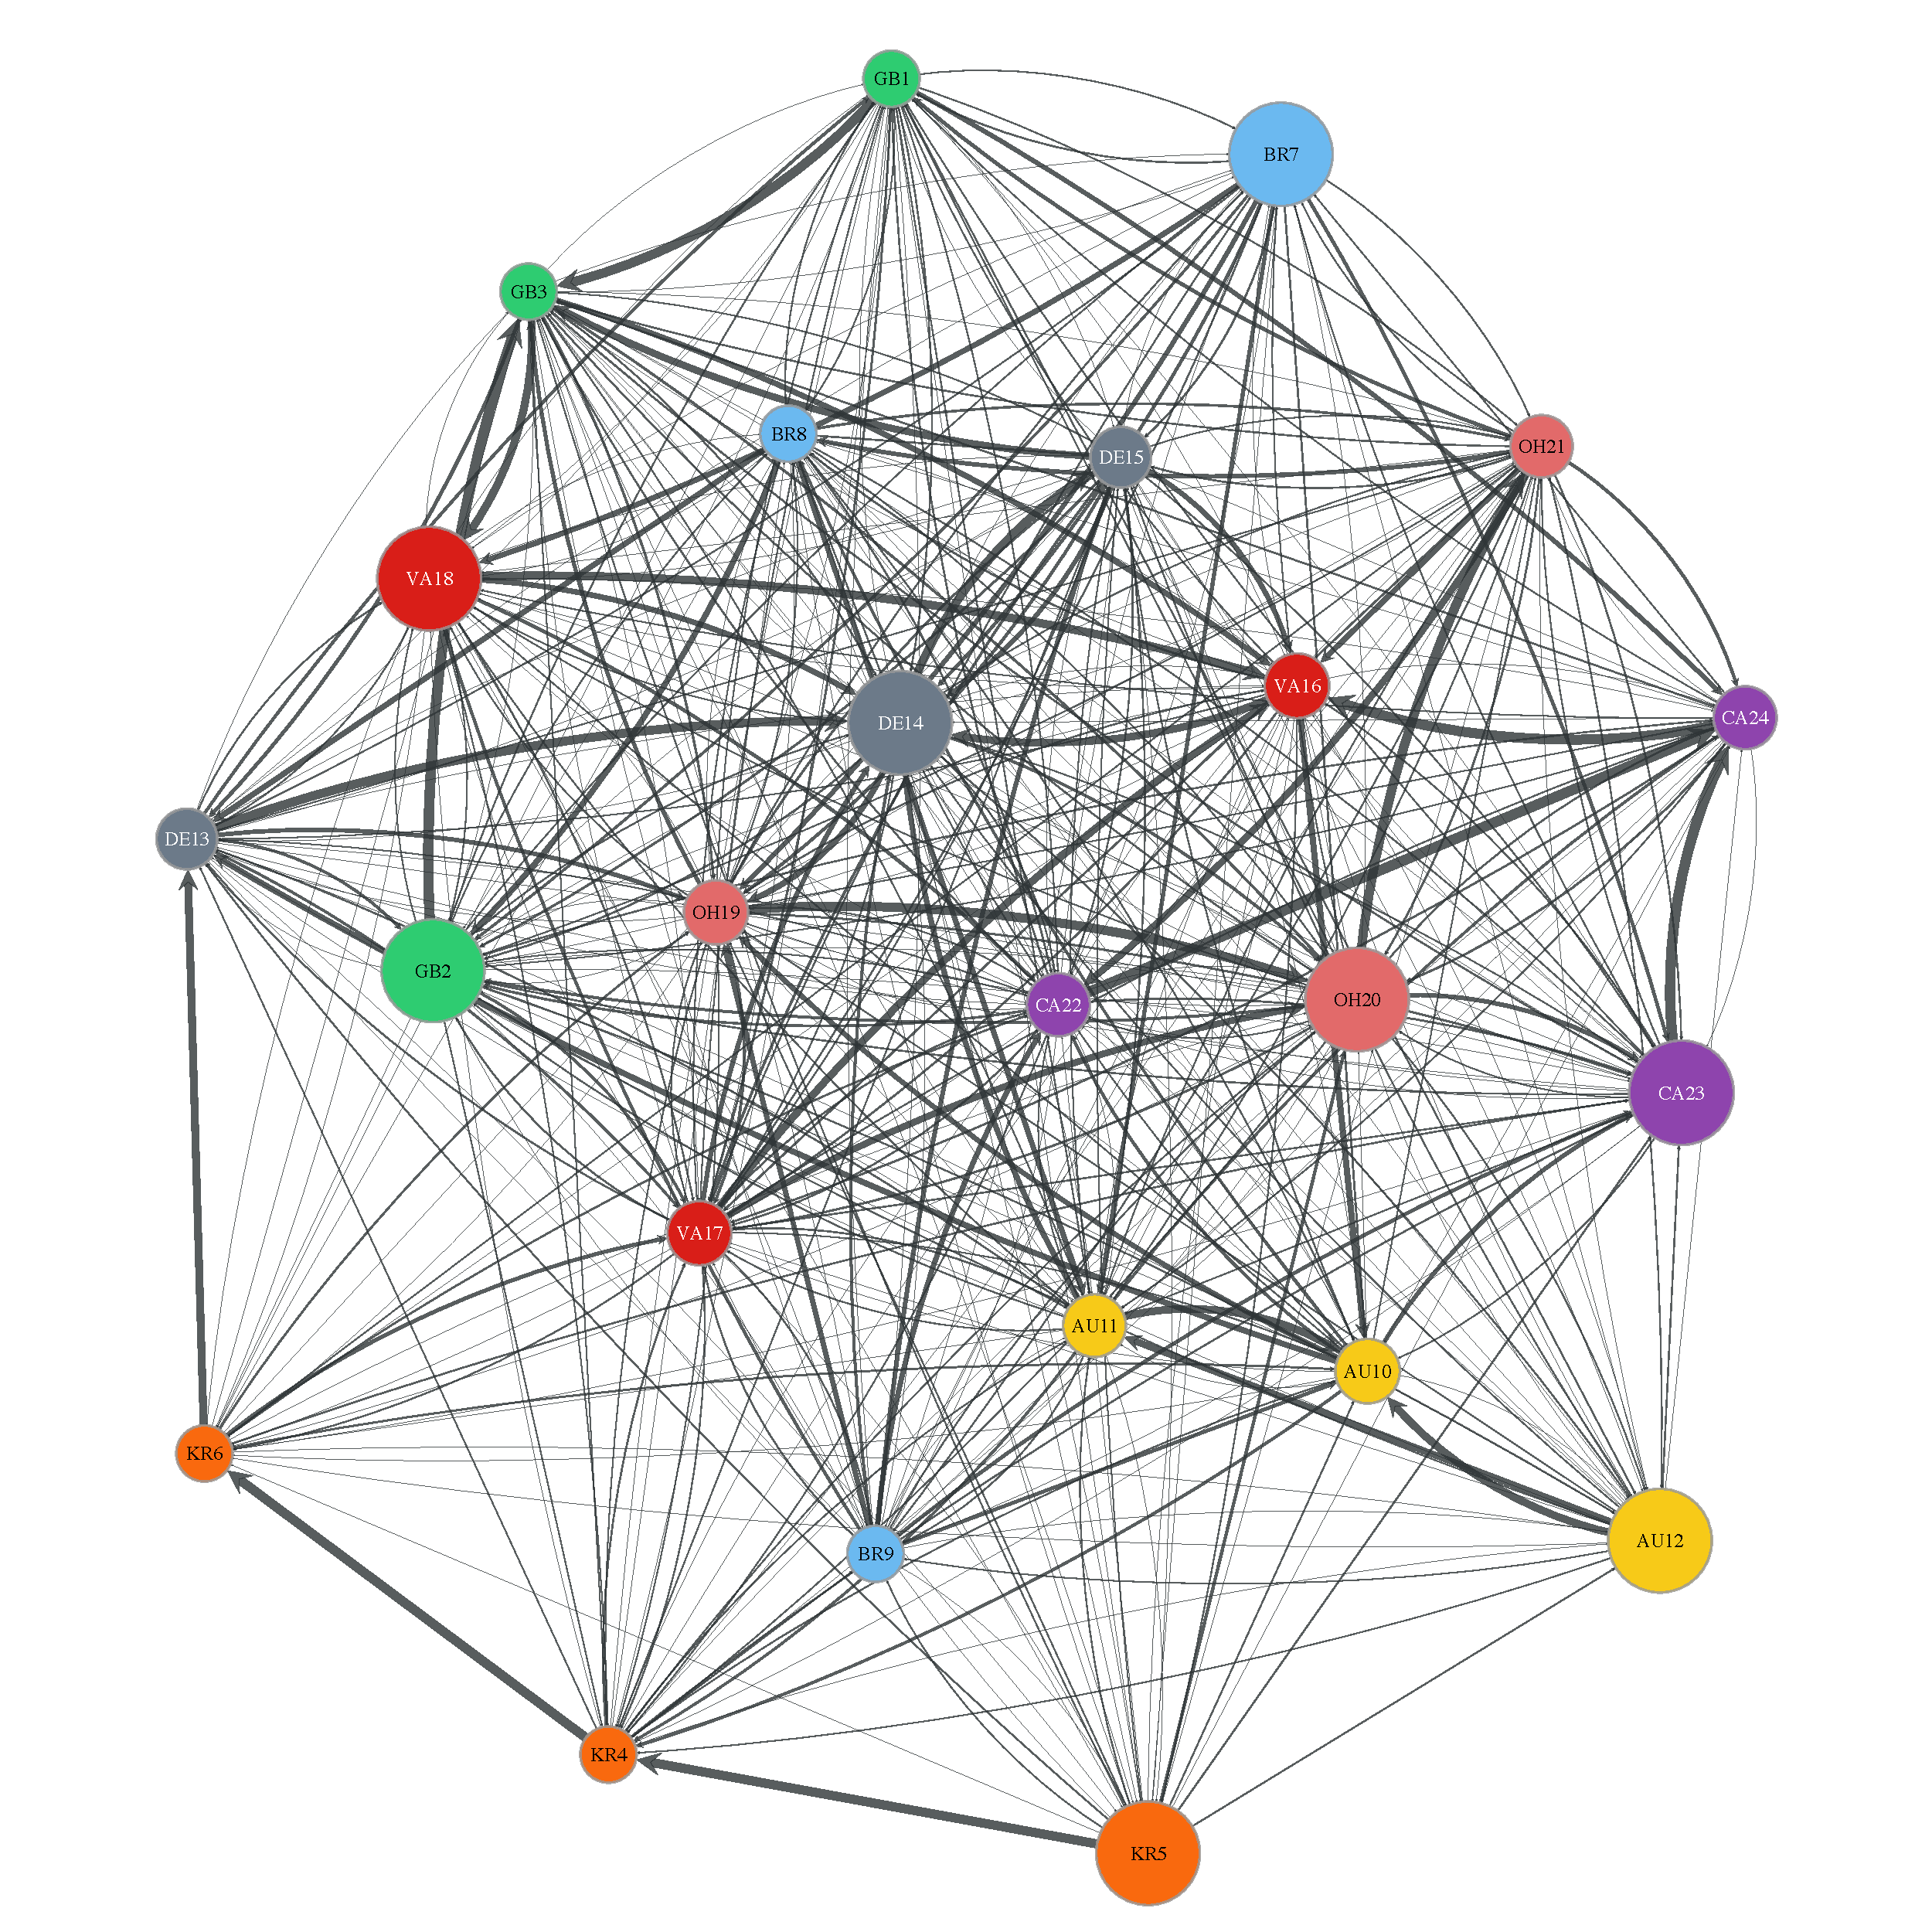
\includegraphics[width=\linewidth]{figures/b-epsilon-greedy-0-1-e2}
      \caption{Epsilon Greedy $\epsilon=0.1$}\label{fig:epsilon_greedy_e1}
    \endminipage
\end{figure*}

\begin{figure*}[t]
    \centering
    \minipage{0.5\textwidth}%
      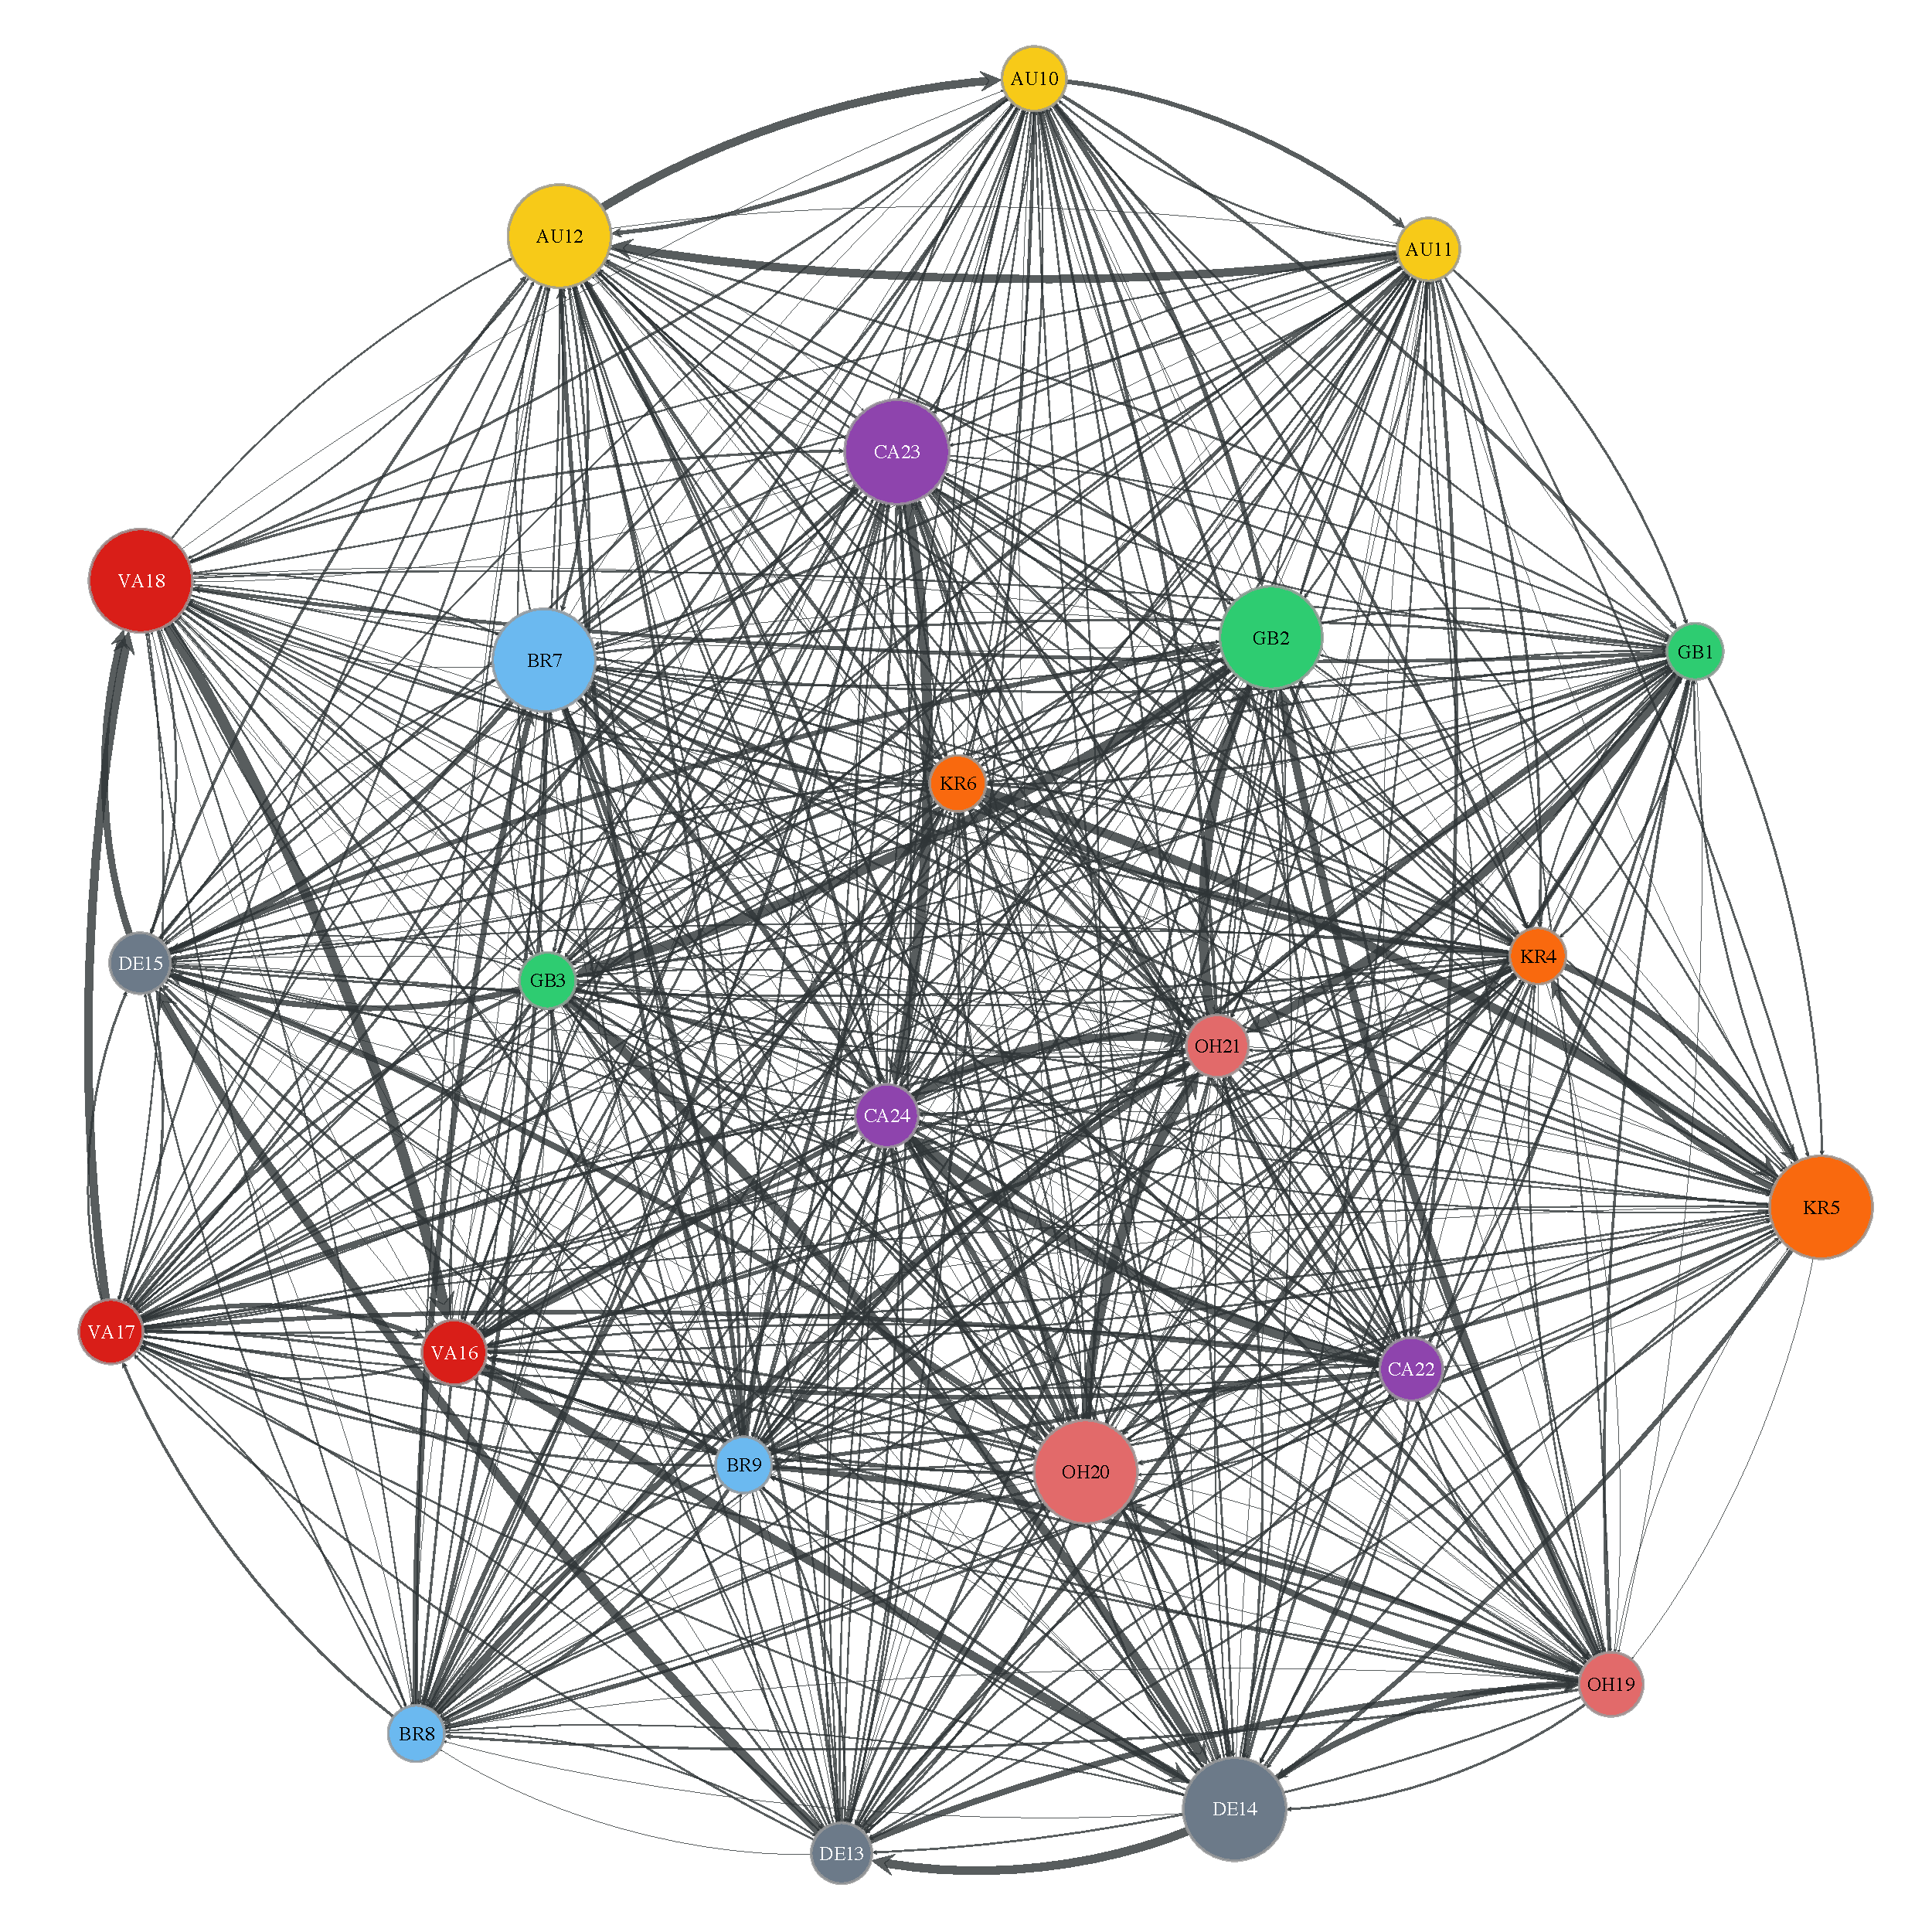
\includegraphics[width=\linewidth]{figures/b-epsilon-greedy-0-2-e3}
      \caption{Epsilon Greedy $\epsilon=0.2$}\label{fig:epsilon_greedy_e2}
  \endminipage\hfill
  \minipage{0.5\textwidth}%
    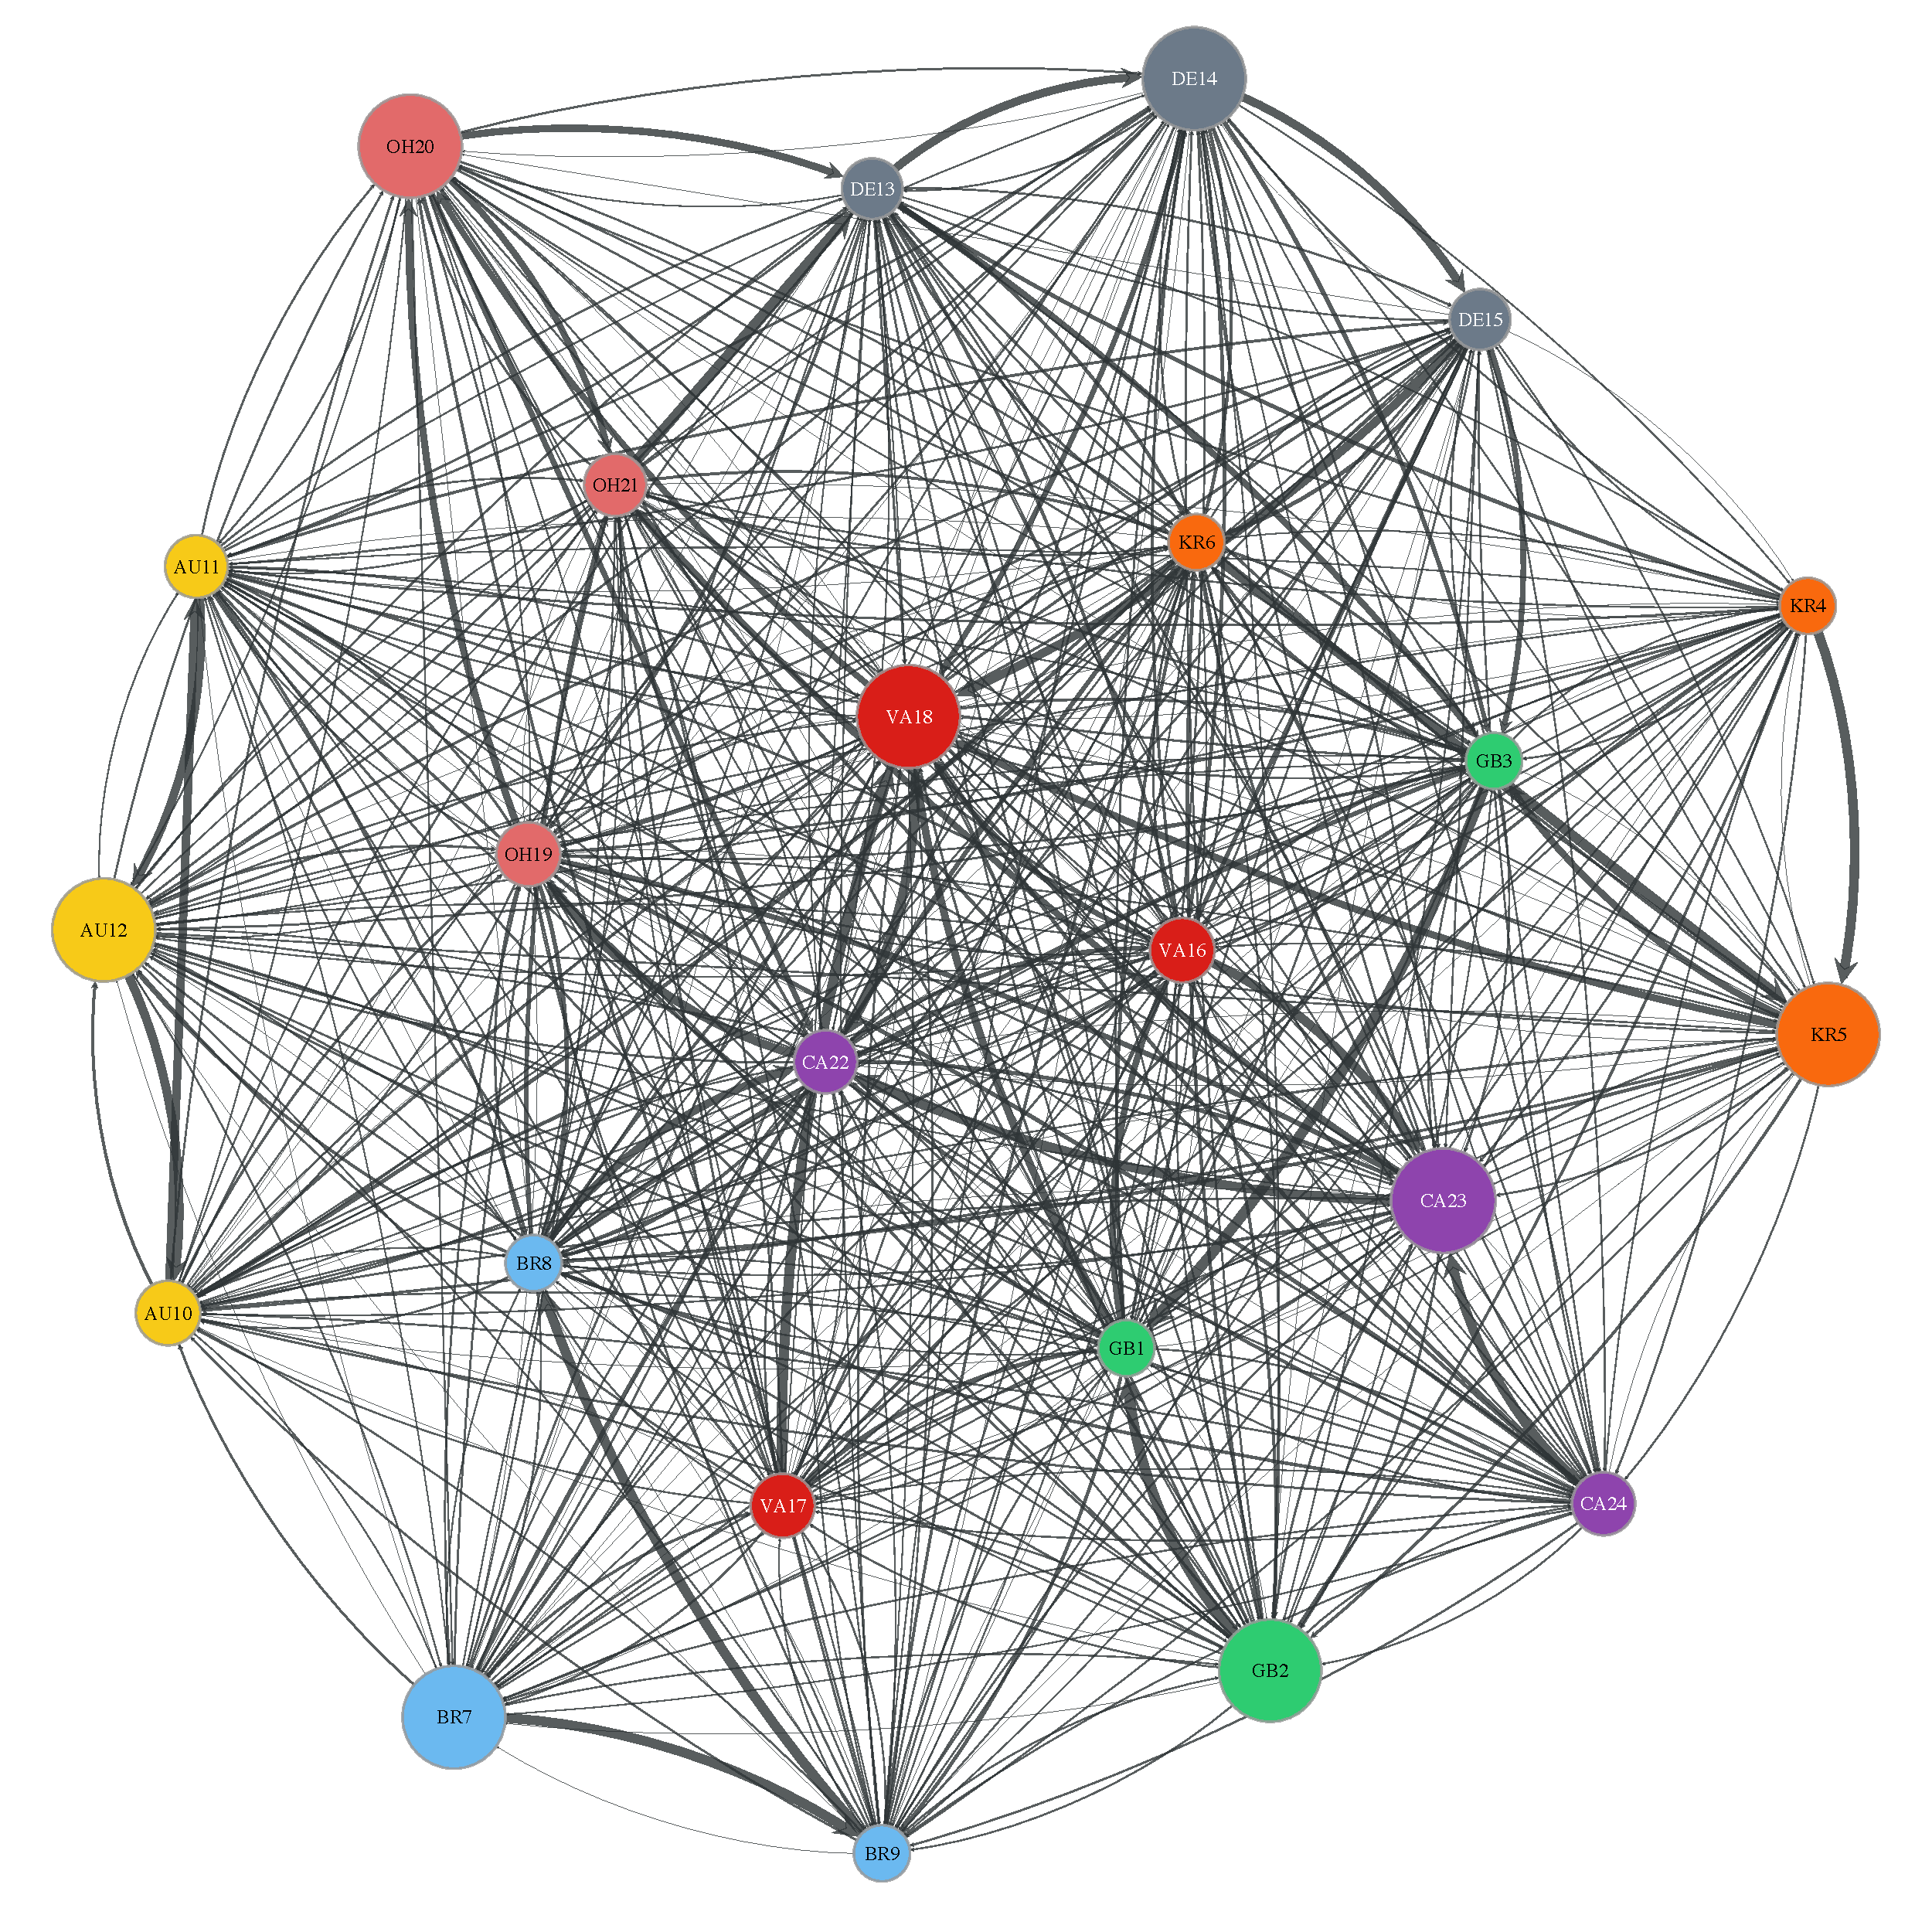
\includegraphics[width=\linewidth]{figures/b-annealing-epsilon-greedy-e5}
    \caption{Annealing Epsilon Greedy}\label{fig:annealing_epsilon}
  \endminipage
\end{figure*}

We have visualized the resulting topologies as network diagrams in
Figure~\ref{fig:uniform_selection} (uniform selection),
Figure~\ref{fig:epsilon_greedy_e1} (epsilon greedy $\epsilon=0.1$),
Figure~\ref{fig:epsilon_greedy_e2} (epsilon greedy $\epsilon=0.2$), and
Figure~\ref{fig:annealing_epsilon} (annealing epsilon).
Each network diagram shows each replica as a vertex, colored by region e.g.
purple is California, light blue is Sao Paulo, Brazil, etc.
Each vertex is also labeled with the 2-character UN country or US state
abbreviation as well as the replica's precedence id.
The size of the vertex represents the number of \texttt{Put} requests that
replica received over the course of the experiment; larger vertices
represent replicas that were colocated with workload generators.
Each edge between vertices represents the total number of successful
synchronizations, the darker and thicker the edge is, the more
synchronizations occurred between the two replicas.
Edges are directed, the source of the edge is the replica that initiated
anti-entropy with the target of the edge.

Comparing the resulting networks, it is easy to see that more defined
topologies result from the bandit-based approaches.
The uniform selection network is simply a hairball of connections with
a limited number of synchronizations.
Clear optimal connections have emerged with the bandit strategies, dark
lines represent extremely successful synchronization connections between
replicas, while light lines represent synchronization pairs that are
selected less frequently.
We posit that fewer edges in the graph represents a more stable network;
the fewer synchronization pairs that are selected, the less noise that
occurs from selecting a peer that is in a similar state.

\section*{Discussion}

To achieve stronger eventual consistency, the visibility latency
of a system replicated with anti-entropy must be reduced.
We believe that this can be achieved with two primary goals: increasing
the number of successful synchronizations and maximizing the the number
of local and regional synchronizations such that the average latency of
anti-entropy sessions is as low as possible.
These goals must also be tempered against other requirements, such as
fault and partition tolerance, a deterministic anti-entropy solution that
ensures the system will become consistent eventually, and load balancing
the synchronization workload evenly across all replicas.

Bandit based approaches to peer selection clearly reduce noise inherent
in uniform random selection as shown in Figure~\ref{fig:system_rewards},
the bandit algorithms achieve better rewards over time because peers
are selected that are more likely to have an update to synchronize.
Moreover, based on the network diagrams shown in
Figures~\ref{fig:uniform_selection}-\ref{fig:annealing_epsilon}, this is
not the result of one or two replicas becoming primary syncs: most
replicas have only one or two dark in-edges meaning that most replicas
are only the most valuable peers for one or two other replicas.
At the same time, the rewards using a bandit approach, while clearly better
than the uniform case, are not significantly better.
Future work to explore the reward function in detail may help to adjust
the reward curves more significantly.
Additionally the inclusion of penalties (negative rewards) might also make
the system faster to adjust to a high quality topology.
Future work must also show an increase in consistency by demonstrating a
reduced number of stale reads and forked writes.

As for localization, there does appear to be a natural inclination for
replicas that are geographically proximate to be a more likely selection.
In Figure~\ref{fig:epsilon_greedy_e2}, replicas in Seoul (orange), Virginia
(red), Sydney (yellow), California (purple), and Frankfurt (grey) all
prioritize local connections.
Regionally, this same figure shows strong links such as those between Ohio
and California (\texttt{OH21} $\rightarrow$ \texttt{CA24}) or Frankfurt and
London (\texttt{GB3} $\rightarrow$ \texttt{DE14}).
Replicas such as \texttt{OH21} and \texttt{DE14} appear to be hubs that
specialize in cross-region collaboration.
Unfortunately there does also seem to be an isolating effect, for example
Sydney (yellow) appears to have no significant out of region synchronization
partners.
Multi-stage bandits might be used to create a tiered reward system to
specifically adjust the selection of local, regional, and global peers.
Other strategies such as upper confidence bounds, softmax, or Bayesian
selection may also create more robust localization.

Finally, and perhaps most significantly, the experiments conducted in
this paper were on a static workload; future work must explore dynamic
workloads with changing access patterns to more closely simulate real
world scenarios.
While bandit algorithms are considered online algorithms that do respond
to changing conditions, the epsilon greedy strategy can be slow to change
since it prefers to exploit high-value arms.
Contextual bandits use side information in addition to rewards to make
selection decisions, and there is current research in exploring contextual
bandits in dynamic worlds that may be applicable.
Other strategies such as periodic reseting of the values may incur a small
cost to explore the best anti-entropy topology, but could respond to changing
access patterns or conditions in a meaningful way.

\section*{Conclusion}

In this paper we have presented a novel approach to peer selection during
anti-entropy by replacing uniform random selection with multi-armed bandits.
Multi-armed bandits consider the historical reward obtained from
synchronization with a peer, defined by the number of objects synchronized
and the latency of RPCs, when making a selection.
Bandits balance the exploitation of a known high-value synchronization
peer with the exploration of possibly better peers or the impact of
failures or partitions.
The end result is a replication network that is not only unperturbed by noise
due to randomness, but also capable of more efficiently propagating updates.

In an eventually consistent system, efficient propagation of updates is
directly tied to higher consistency.
By reducing visibility latency, the likelihood of a stale read decreases,
which is the primary source of inconsistency in a highly available system.
Future work will consider different reward functions, different selection
strategies, dynamic environments, and how the priorities of system designers
can be embedded into rewards.
We will also specifically explore in detail the effect of adaptive systems
on consistency.

We believe that the results presented show a promising start to a renewed
investigation of highly available distributed storage systems in novel
network environments, particularly those that span the globe.
Specifically, this work is part of a larger exploration of adaptive,
globally distributed data systems that federate consistency levels to provide
stronger guarantees~\cite{bengfort_federating_2017}.
Federated consistency combines adaptive eventually consistent systems such as
the one presented in this paper with scaling geo-replicated consensus such as
Hierarchical Consensus~\cite{bengfort_brief_2017} in order to create robust
data systems that are automatically tuned to provide the best availability
and consistency.
Distributed systems that adapt to and learn from their environments and
access patterns, such as the emerging synchronization topologies we observed
in this paper, may form the foundation for the extremely large, extremely
efficient networks of the future.

All code for the key-value store and bandit-based entropy as well as
experimental results is open source and available on GitHub at
\url{https://github.com/bbengfort/honu}.
